% !TEX encoding = UTF-8
% !TEX TS-program = pdflatex
% !TEX root = ../tesi.tex

\newgeometry{a4paper, left=30mm, right=30mm, top=5mm, bottom=30mm}
%**************************************************************
\chapter{Analisi dei requisiti}
\label{cap:analisi-requisiti}
%**************************************************************

\noindent \intro{In questo capitolo viene sposta l'analisi dei requisiti effettuata durante lo \textit{stage}, nella quale vengono descritte le funzionalità tramite i casi d'uso.}\\

\section{Casi d'uso}

\noindent Per lo studio dei casi di utilizzo del prodotto sono stati creati dei diagrammi.
I diagrammi dei casi d'uso (in inglese \emph{\textit{Use Case} Diagram}) sono diagrammi di tipo \textit{\gls{umlg}} dedicati alla descrizione delle funzioni o servizi offerti da un sistema, così come sono percepiti e utilizzati dagli attori che interagiscono col sistema stesso.
Essendo il progetto finalizzato alla creazione di un \textit{tool} per l'automazione di un processo, le interazioni da parte dell'utilizzatore devono essere ovviamente ridotte allo stretto necessario. Per questo motivo i diagrammi dei casi d'uso risultano semplici e in numero ridotto.\\

\noindent A livello formale, i diagrammi dei casi d'uso avranno la seguente forma:
\begin{center}
    \textbf{UC<CodicePadre>.<CodiceFiglio>}
\end{center}
\noindent È importante ribadire come questo formalismo sia gerarchico, ovvero un codice figlio
può essere codice padre di un suo eventuale codice figlio. Possono essere figli le generalizzazioni e i sottocasi d'uso.\\

\noindent Nella figura di seguito verrà illustrato il diagramma del sistema principale con tutti i casi d'uso.
\vspace*{\fill}
\begin{figure}[!h] 
   \centering 
   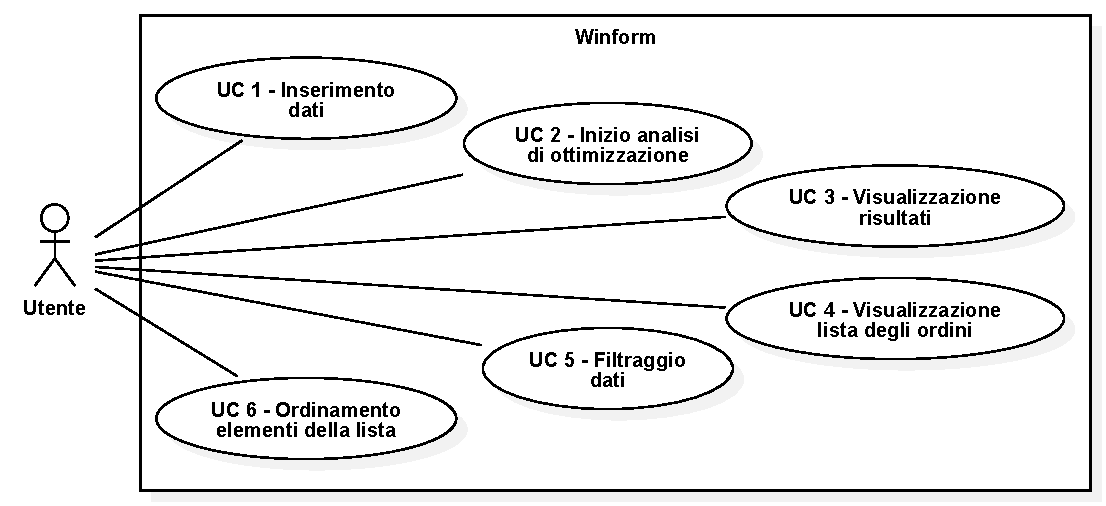
\includegraphics[width=0.91\columnwidth]{usecase/winform.pdf} 
   \caption{Use case - sistema principale}
\end{figure}
\vspace*{\fill}
\newgeometry{a4paper, left=30mm, right=30mm, top=31mm, bottom=30mm}

\noindent \textbf{\large UC 1 - Inserimento dati}
\label{uc:inserimento-dati}
\begin{figure}[!h] 
    \centering 
    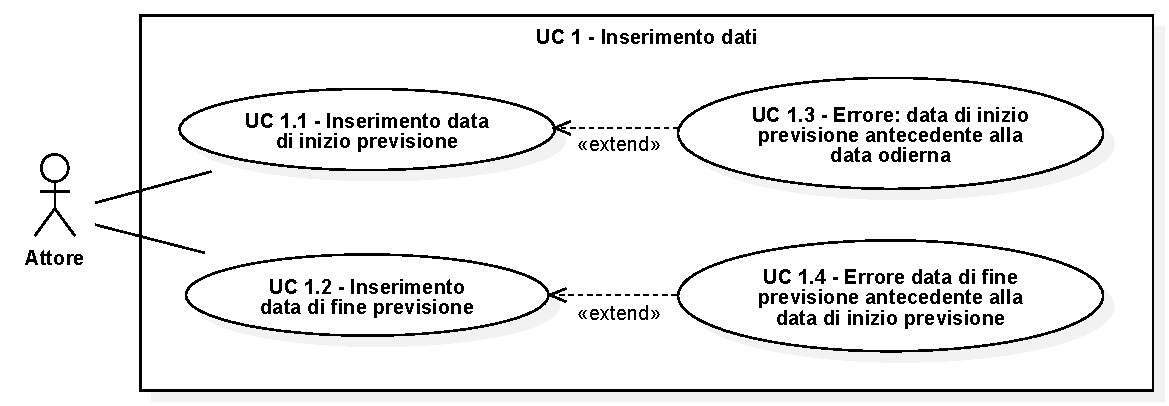
\includegraphics[width=0.95\columnwidth]{usecase/UC 1.pdf} 
    \caption{UC1 - Inserimento dati}
\end{figure}
\begin{itemize}

	\item \textbf{Attori primari: }
		\begin{itemize}
			\item Utente.
		\end{itemize}

	\item \textbf{Precondizione: }\\[0.3cm]
		L'utente è dentro la \textit{form} e non ha ancora inserito alcun dato.

	\item \textbf{Scenario principale: }
		\begin{enumerate}
			\item L'utente inserisce i dati.
		\end{enumerate}
		

	\item \textbf{Postcondizione: }\\[0.3cm]
		L'utente ha inserito i dati correttamente.

\end{itemize}

\vspace{0.4cm}

\noindent \textbf{\large UC 1.1 - Inserimento data di inizio previsione}
\label{uc:inserimento-data-inizio-prev}
\begin{itemize}

	\item \textbf{Attori primari: }
		\begin{itemize}
			\item Utente.
		\end{itemize}

	\item \textbf{Precondizione: }\\[0.3cm]
		L'utente è dentro la \textit{form} e non ha ancora inserito la data di inizio previsione.

	\item \textbf{Scenario principale: }
		\begin{enumerate}
			\item L'utente seleziona la data di inizio previsione.
		\end{enumerate}

	\item \textbf{Postcondizione: }\\[0.3cm]
		L'utente ha inserito la data di inizio previsione correttamente.

	\item \textbf{Scenario alternativo: }
		\begin{itemize}
		    \item La \textit{form} segnala un errore di immissione dati (\hyperref[uc:err-inserimento-data-inizio-prev]{UC 1.3}).
		\end{itemize}

\end{itemize}

\vspace{0.4cm}


\newpage

\noindent \textbf{\large UC 1.2 - Inserimento data di fine previsione}
\label{uc:inserimento-data-fine-prev}
\begin{itemize}

	\item \textbf{Attori primari: }
		\begin{itemize}
			\item Utente.
		\end{itemize}

	\item \textbf{Precondizione: }\\[0.3cm]
		L'utente è dentro la \textit{form} e non ha ancora inserito la data di fine previsione.

	\item \textbf{Scenario principale: }
		\begin{enumerate}
			\item L'utente inserisce la data di fine previsione;
		\end{enumerate}

	\item \textbf{Postcondizione: }\\[0.3cm]
		L'utente ha inserito la data di fine previsione correttamente.

	\item \textbf{Scenario alternativo: }
		\begin{itemize}
		    \item La \textit{form} segnala un errore di immissione dati (\hyperref[uc:err-inserimento-data-fine-prev]{UC 1.4}).
		\end{itemize}

\end{itemize}

\vspace{0.4cm}

\noindent \textbf{\large UC 1.3 - Errore: data di inizio previsione antecedente alla data odierna}
\label{uc:err-inserimento-data-inizio-prev}
\begin{itemize}

	\item \textbf{Attori primari: }
		\begin{itemize}
			\item Utente.
		\end{itemize}

	\item \textbf{Precondizione: }\\[0.3cm]
		L'utente è dentro la \textit{form} e ha inserito una data di inizio previsione antecedente
		alla data odierna.

	\item \textbf{Scenario principale: }
		\begin{enumerate}
			\item L'utente conferma la data di inizio previsione;
			\item L'utente visualizza un errore generato dalla \textit{form}.
		\end{enumerate}
		

	\item \textbf{Postcondizione: }\\[0.3cm]
		L'utente viene avvisato dell'errore di immissione.

\end{itemize}

\vspace{0.4cm}

\noindent \textbf{\large UC 1.4 - Errore: data di fine previsione antecedente alla data di \\\hspace*{56pt}inizio previsione}
\label{uc:err-inserimento-data-fine-prev}
\begin{itemize}

	\item \textbf{Attori primari: }
		\begin{itemize}
			\item Utente.
		\end{itemize}

	\item \textbf{Precondizione: }\\[0.3cm]
		L'utente è dentro la \textit{form} e ha inserito una data di fine previsione antecedente
		alla data odierna.

	\item \textbf{Scenario principale: }
		\begin{enumerate}
			\item L'utente conferma la data di fine previsione;
			\item L'utente visualizza un errore generato dalla \textit{form}.
		\end{enumerate}
		

	\item \textbf{Postcondizione: }\\[0.3cm]
		L'utente viene avvisato dell'errore di immissione.

\end{itemize}

\vspace{0.4cm}

\noindent \textbf{\large UC 2 - Inizio analisi di ottimizzazione}
\label{uc:inizio-analisi-ottimizzazione}
\begin{itemize}

	\item \textbf{Attori primari: }
		\begin{itemize}
			\item Utente.
		\end{itemize}

	\item \textbf{Precondizione: }\\[0.3cm]
		L'utente è dentro la \textit{form} e ha inserito una data di inizio e fine previsione valide.

	\item \textbf{Scenario principale: }
		\begin{enumerate}
			\item L'utente conferma l'inizio dell'analisi di ottimizzazione.
		\end{enumerate}
		

	\item \textbf{Postcondizione: }\\[0.3cm]
		L'utente ha effettuato l'analisi di ottimizzazione per le date di inizio e fine previsione e visualizza correttamente i
		risultati (\hyperref[uc:visualizzazione-risultati]{UC 3}).

\end{itemize}

\vspace{0.4cm}

\noindent \textbf{\large UC 3 - Visualizzazione risultati}
\label{uc:visualizzazione-risultati}
\begin{figure}[!h] 
    \centering 
    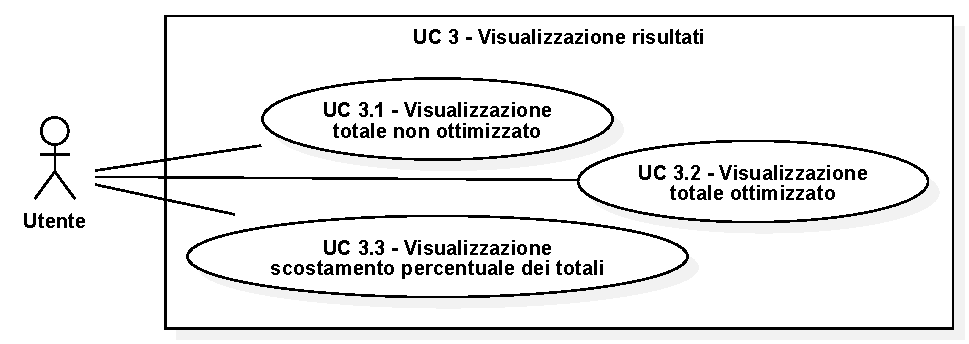
\includegraphics[width=0.95\columnwidth]{usecase/UC 3.pdf} 
    \caption{UC3 - Visualizzazione risultati}
\end{figure}
\begin{itemize}

	\item \textbf{Attori primari: }
		\begin{itemize}
			\item Utente.
		\end{itemize}

	\item \textbf{Precondizione: }\\[0.3cm]
		L'utente è dentro la \textit{form} e ha effettuato l'analisi di ottimizzazione correttamente.

	\item \textbf{Scenario principale: }
		\begin{enumerate}
			\item L'utente visualizza il totale non ottimizzato (\hyperref[uc:visualizzazione-totale-non-ottimizzato]{UC 3.1});
			\item L'utente visualizza il totale ottimizzato (\hyperref[uc:visualizzazione-totale-ottimizzato]{UC 3.2});
			\item L'utente visualizza lo scostamento percentuale dei totali (\hyperref[uc:visualizzazione-scostamento-percentuale-totali]{UC 3.3}).
		\end{enumerate}
		

	\item \textbf{Postcondizione: }\\[0.3cm]
		L'utente visualizza correttamente tutti i risultati.

\end{itemize}

\vspace{0.4cm}

\newpage

\noindent \textbf{\large UC 3.1 - Visualizzazione totale non ottimizzato}
\label{uc:visualizzazione-totale-non-ottimizzato}
\begin{itemize}

	\item \textbf{Attori primari: }
		\begin{itemize}
			\item Utente.
		\end{itemize}

	\item \textbf{Precondizione: }\\[0.3cm]
		L'utente è dentro la \textit{form} e ha effettuato l'analisi di ottimizzazione correttamente.

	\item \textbf{Scenario principale: }
		\begin{enumerate}
			\item L'utente visualizza il totale non ottimizzato.
		\end{enumerate}
		

	\item \textbf{Postcondizione: }\\[0.3cm]
		L'utente visualizza correttamente il totale non ottimizzato.

\end{itemize}

\vspace{0.4cm}

\noindent \textbf{\large UC 3.2 - Visualizzazione totale ottimizzato}
\label{uc:visualizzazione-totale-ottimizzato}
\begin{itemize}

	\item \textbf{Attori primari: }
		\begin{itemize}
			\item Utente.
		\end{itemize}

	\item \textbf{Precondizione: }\\[0.3cm]
		L'utente è dentro la \textit{form} e ha effettuato l'analisi di ottimizzazione correttamente.

	\item \textbf{Scenario principale: }
		\begin{enumerate}
			\item L'utente visualizza il totale ottimizzato.
		\end{enumerate}
		

	\item \textbf{Postcondizione: }\\[0.3cm]
		L'utente visualizza correttamente il totale ottimizzato.

\end{itemize}

\vspace{0.4cm}

\noindent \textbf{\large UC 3.3 - Visualizzazione scostamento percentuale dei totali}
\label{uc:visualizzazione-scostamento-percentuale-totali}
\begin{itemize}

	\item \textbf{Attori primari: }
		\begin{itemize}
			\item Utente.
		\end{itemize}

	\item \textbf{Precondizione: }\\[0.3cm]
		L'utente è dentro la \textit{form} e ha effettuato l'analisi di ottimizzazione correttamente.

	\item \textbf{Scenario principale: }
		\begin{enumerate}
			\item L'utente visualizza lo scostamento percentuale dei totali.
		\end{enumerate}
		

	\item \textbf{Postcondizione: }\\[0.3cm]
		L'utente visualizza correttamente lo scostamento percentuale dei totali.

\end{itemize}

\vspace{0.4cm}

\newpage

\noindent \textbf{\large UC 4 - Visualizzazione lista degli ordini}
\begin{figure}[!h] 
    \centering 
    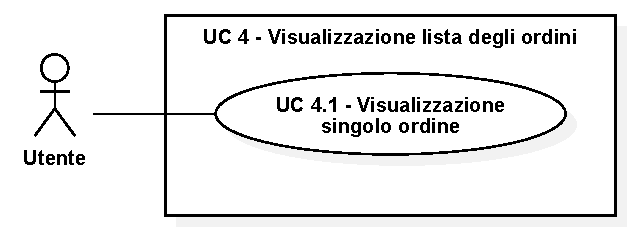
\includegraphics[width=0.65\columnwidth]{usecase/UC 4.pdf} 
    \caption{UC4 - Visualizzazione lista degli ordini}
\end{figure}
\label{uc:visualizzazione-lista-ordini}
\begin{itemize}

	\item \textbf{Attori primari: }
		\begin{itemize}
			\item Utente.
		\end{itemize}

	\item \textbf{Precondizione: }\\[0.3cm]
		L'utente è dentro la \textit{form} e ha effettuato l'analisi di ottimizzazione correttamente.

	\item \textbf{Scenario principale: }
		\begin{enumerate}
			\item L'utente visualizza la lista degli ordini da effettuare.
		\end{enumerate}
		

	\item \textbf{Postcondizione: }\\[0.3cm]
		L'utente visualizza correttamente la lista degli ordini da effettuare.

\end{itemize}

\vspace{0.4cm}

\vspace*{\fill}

\noindent \textbf{\large UC 4.1 - Visualizzazione singolo ordine}
\begin{figure}[!h] 
    \centering 
    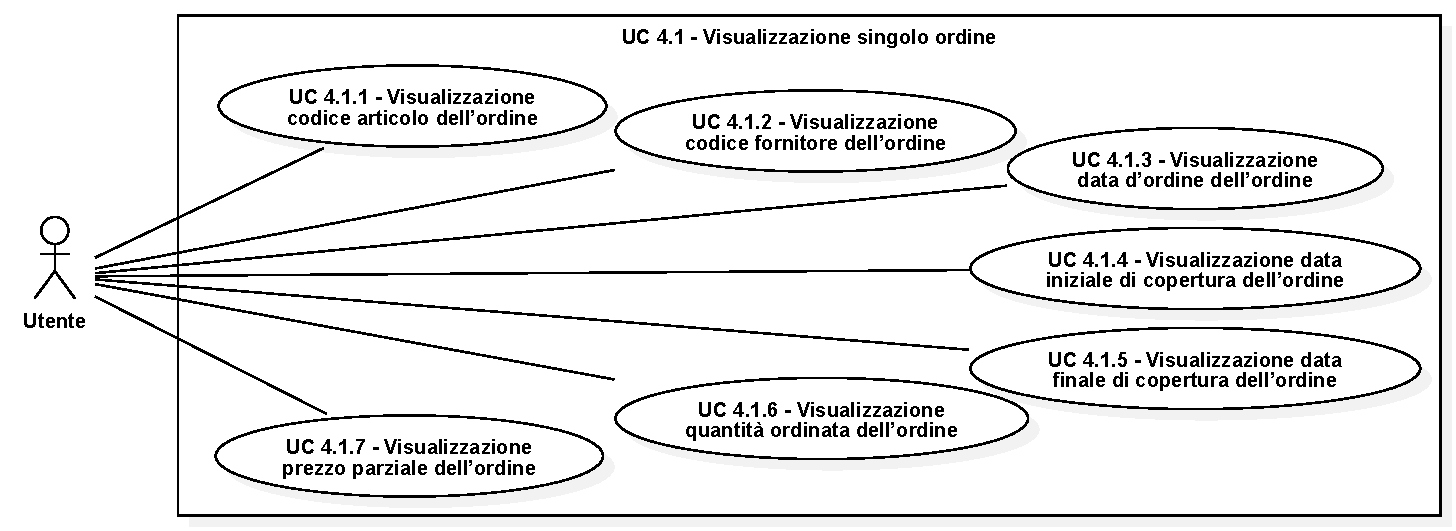
\includegraphics[width=0.95\columnwidth]{usecase/UC 4.1.pdf} 
    \caption{UC4.1 - Visualizzazione singolo ordine}
\end{figure}
\label{uc:visualizzazione-singolo-ordine}
\begin{itemize}

	\item \textbf{Attori primari: }
		\begin{itemize}
			\item Utente.
		\end{itemize}

	\item \textbf{Precondizione: }\\[0.3cm]
		L'utente visualizza correttamente la lista degli ordini.
		
	\vspace*{\fill}

		\newpage
	
	\item \textbf{Scenario principale: }
		\begin{enumerate}
			\item L'utente visualizza il singolo ordine con tutte le informazioni tra cui:
			\begin{itemize}
				\item codice articolo (\hyperref[uc:visualizzazione-codice-articolo]{UC 4.1.1});
				\item codice fornitore (\hyperref[uc:visualizzazione-codice-fornitore]{UC 4.1.2});
				\item data d'ordine (\hyperref[uc:visualizzazione-data-ordine]{UC 4.1.3});
				\item data iniziale di copertura (\hyperref[uc:visualizzazione-data-iniziale-copertura]{UC 4.1.4});
				\item data finale di copertura (\hyperref[uc:visualizzazione-data-finale-copertura]{UC 4.1.5});
				\item quantità ordinata (\hyperref[uc:visualizzazione-quantita-ordinata]{UC 4.1.6});
				\item prezzo parziale (\hyperref[uc:visualizzazione-prezzo-parziale-ord]{UC 4.1.7}).
			\end{itemize}.
		\end{enumerate}
		

	\item \textbf{Postcondizione: }\\[0.3cm]
		L'utente visualizza correttamente il singolo ordine.

\end{itemize}

\vspace{0.4cm}

\noindent \textbf{\large UC 4.1.1 - Visualizzazione codice articolo dell'ordine}
\label{uc:visualizzazione-codice-articolo}
\begin{itemize}

	\item \textbf{Attori primari: }
		\begin{itemize}
			\item Utente.
		\end{itemize}

	\item \textbf{Precondizione: }\\[0.3cm]
		L'utente visualizza correttamente il singolo ordine.

	\item \textbf{Scenario principale: }
		\begin{enumerate}
			\item L'utente visualizza il codice articolo del singolo ordine.
		\end{enumerate}
		

	\item \textbf{Postcondizione: }\\[0.3cm]
		L'utente visualizza correttamente il codice articolo del singolo ordine.

\end{itemize}

\vspace{0.4cm}

\noindent \textbf{\large UC 4.1.2 - Visualizzazione codice fornitore dell'ordine}
\label{uc:visualizzazione-codice-fornitore}
\begin{itemize}

	\item \textbf{Attori primari: }
		\begin{itemize}
			\item Utente.
		\end{itemize}

	\item \textbf{Precondizione: }\\[0.3cm]
		L'utente visualizza correttamente il singolo ordine.

	\item \textbf{Scenario principale: }
		\begin{enumerate}
			\item L'utente visualizza il codice fornitore del singolo ordine.
		\end{enumerate}
		

	\item \textbf{Postcondizione: }\\[0.3cm]
		L'utente visualizza correttamente il codice fornitore del singolo ordine.

\end{itemize}

\vspace{0.4cm}

\newpage

\noindent \textbf{\large UC 4.1.3 - Visualizzazione data d'ordine dell'ordine}
\label{uc:visualizzazione-data-ordine}
\begin{itemize}

	\item \textbf{Attori primari: }
		\begin{itemize}
			\item Utente.
		\end{itemize}

	\item \textbf{Precondizione: }\\[0.3cm]
		L'utente visualizza correttamente il singolo ordine.

	\item \textbf{Scenario principale: }
		\begin{enumerate}
			\item L'utente visualizza la data d'ordine del singolo ordine.
		\end{enumerate}
		

	\item \textbf{Postcondizione: }\\[0.3cm]
		L'utente visualizza correttamente la data d'ordine del singolo ordine.

\end{itemize}

\vspace{0.4cm}

\noindent \textbf{\large UC 4.1.4 - Visualizzazione data iniziale di copertura dell'ordine}
\label{uc:visualizzazione-data-iniziale-copertura}
\begin{itemize}

	\item \textbf{Attori primari: }
		\begin{itemize}
			\item Utente.
		\end{itemize}

	\item \textbf{Precondizione: }\\[0.3cm]
		L'utente visualizza correttamente il singolo ordine.

	\item \textbf{Scenario principale: }
		\begin{enumerate}
			\item L'utente visualizza la data iniziale di copertura del singolo ordine.
		\end{enumerate}
		

	\item \textbf{Postcondizione: }\\[0.3cm]
		L'utente visualizza correttamente la data iniziale di copertura del singolo ordine.

\end{itemize}

\vspace{0.4cm}

\noindent \textbf{\large UC 4.1.5 - Visualizzazione data finale di copertura dell'ordine}
\label{uc:visualizzazione-data-finale-copertura}
\begin{itemize}

	\item \textbf{Attori primari: }
		\begin{itemize}
			\item Utente.
		\end{itemize}

	\item \textbf{Precondizione: }\\[0.3cm]
		L'utente visualizza correttamente il singolo ordine.

	\item \textbf{Scenario principale: }
		\begin{enumerate}
			\item L'utente visualizza la data finale di copertura del singolo ordine.
		\end{enumerate}
		

	\item \textbf{Postcondizione: }\\[0.3cm]
		L'utente visualizza correttamente la data finale di copertura del singolo ordine.

\end{itemize}

\vspace{0.4cm}

\newpage

\noindent \textbf{\large UC 4.1.6 - Visualizzazione quantità ordinata dell'ordine}
\label{uc:visualizzazione-quantita-ordinata}
\begin{itemize}

	\item \textbf{Attori primari: }
		\begin{itemize}
			\item Utente.
		\end{itemize}

	\item \textbf{Precondizione: }\\[0.3cm]
		L'utente visualizza correttamente il singolo ordine.

	\item \textbf{Scenario principale: }
		\begin{enumerate}
			\item L'utente visualizza la quantità ordinata del singolo ordine.
		\end{enumerate}
		

	\item \textbf{Postcondizione: }\\[0.3cm]
		L'utente visualizza correttamente la quantità ordinata del singolo ordine.

\end{itemize}

\vspace{0.4cm}

\noindent \textbf{\large UC 4.1.7 - Visualizzazione prezzo parziale dell'ordine}
\label{uc:visualizzazione-prezzo-parziale-ord}
\begin{itemize}

	\item \textbf{Attori primari: }
		\begin{itemize}
			\item Utente.
		\end{itemize}

	\item \textbf{Precondizione: }\\[0.3cm]
		L'utente visualizza correttamente il singolo ordine.

	\item \textbf{Scenario principale: }
		\begin{enumerate}
			\item L'utente visualizza il prezzo parziale del singolo ordine.
		\end{enumerate}
		

	\item \textbf{Postcondizione: }\\[0.3cm]
		L'utente visualizza correttamente il prezzo parziale del singolo ordine.

\end{itemize}

\vspace{0.4cm}

\noindent \textbf{\large UC 5 - Filtraggio dati}
\label{uc:filtraggio-dati}
\begin{figure}[!h] 
    \centering 
    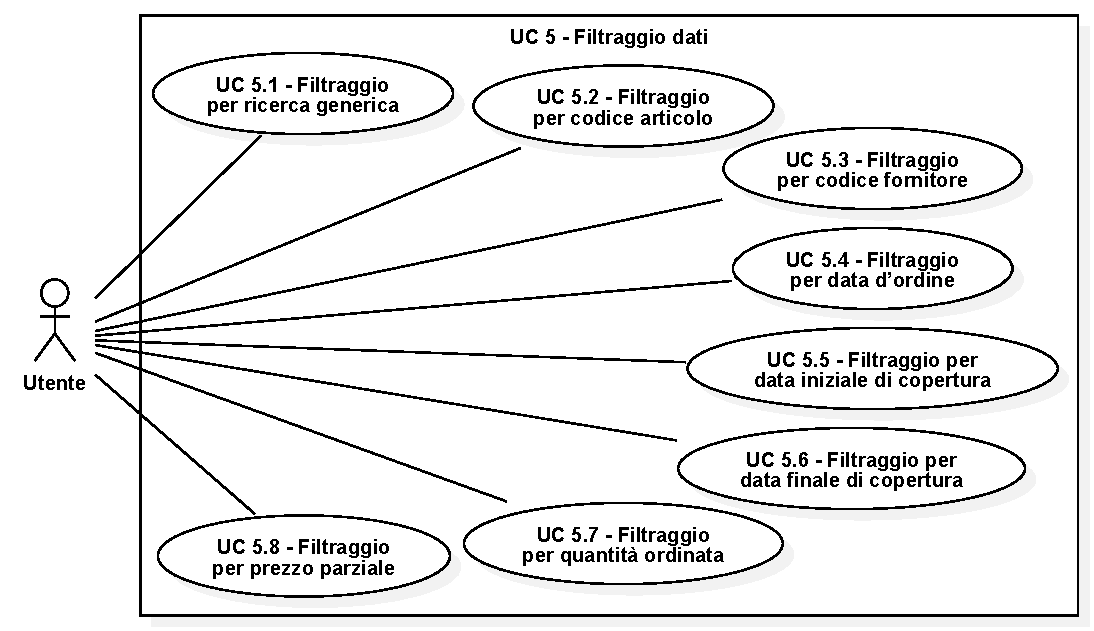
\includegraphics[width=0.95\columnwidth]{usecase/UC 5.pdf} 
    \caption{UC 5 - Filtraggio dati}
\end{figure}
\begin{itemize}

	\item \textbf{Attori primari: }
		\begin{itemize}
			\item Utente.
		\end{itemize}

	\item \textbf{Precondizione: }\\[0.3cm]
		L'utente visualizza correttamente la lista degli ordini.

	\item \textbf{Scenario principale: }
		\begin{enumerate}
			\item L'utente sceglie uno o più filtri da applicare alla lista.\\
			In particolare le tipologie di filtro disponibili sono per:
			\begin{itemize}
				\item codice articolo (\hyperref[uc:filtraggio-codice-articolo]{UC 5.1});
				\item codice articolo (\hyperref[uc:filtraggio-codice-articolo]{UC 5.2});
				\item codice fornitore (\hyperref[uc:filtraggio-codice-fornitore]{UC 5.3});
				\item data d'ordine (\hyperref[uc:filtraggio-data-ordine]{UC 5.4});
				\item data iniziale di copertura (\hyperref[uc:filtraggio-data-iniziale-copertura]{UC 5.5});
				\item data finale di copertura (\hyperref[uc:filtraggio-data-finale-copertura]{UC 5.6});
				\item quantità ordinata (\hyperref[uc:filtraggio-quantita-ordinata]{UC 5.7});
				\item prezzo parziale (\hyperref[uc:filtraggio-prezzo-parziale-ord]{UC 5.8}).
			\end{itemize}
		\end{enumerate}
		

	\item \textbf{Postcondizione: }\\[0.3cm]
		L'utente visualizza correttamente tutti gli elementi che soddisfano i filtri applicati.

\end{itemize}

\vspace{0.4cm}

\noindent \textbf{\large UC 5.1 - Filtraggio per ricerca generica}
\label{uc:filtraggio-ricerca-generica}
\begin{itemize}

	\item \textbf{Attori primari: }
		\begin{itemize}
			\item Utente.
		\end{itemize}

	\item \textbf{Precondizione: }\\[0.3cm]
		L'utente visualizza correttamente la lista degli ordini.

	\item \textbf{Scenario principale: }
		\begin{enumerate}
			\item L'utente filtra uno o più ordini tramite una ricerca generica.
		\end{enumerate}
		

	\item \textbf{Postcondizione: }\\[0.3cm]
		L'utente visualizza correttamente tutti gli elementi che soddisfano il filtro.

\end{itemize}

\vspace{0.4cm}

\noindent \textbf{\large UC 5.2 - Filtraggio per codice articolo}
\label{uc:filtraggio-codice-articolo}
\begin{itemize}

	\item \textbf{Attori primari: }
		\begin{itemize}
			\item Utente.
		\end{itemize}

	\item \textbf{Precondizione: }\\[0.3cm]
		L'utente visualizza correttamente la lista degli ordini.

	\item \textbf{Scenario principale: }
		\begin{enumerate}
			\item L'utente filtra uno o più ordini per codice articolo.
		\end{enumerate}
		

	\item \textbf{Postcondizione: }\\[0.3cm]
		L'utente visualizza correttamente tutti gli elementi che soddisfano il filtro.

\end{itemize}

\vspace{0.4cm}

\noindent \textbf{\large UC 5.3 - Filtraggio per codice fornitore}
\label{uc:filtraggio-codice-fornitore}
\begin{itemize}

	\item \textbf{Attori primari: }
		\begin{itemize}
			\item Utente.
		\end{itemize}

	\item \textbf{Precondizione: }\\[0.3cm]
		L'utente visualizza correttamente la lista degli ordini.

	\item \textbf{Scenario principale: }
		\begin{enumerate}
			\item L'utente filtra uno o più ordini per codice fornitore.
		\end{enumerate}
		

	\item \textbf{Postcondizione: }\\[0.3cm]
		L'utente visualizza correttamente tutti gli elementi che soddisfano il filtro.

\end{itemize}

\vspace{0.4cm}

\noindent \textbf{\large UC 5.4 - Filtraggio per data d'ordine}
\label{uc:filtraggio-data-ordine}
\begin{itemize}

	\item \textbf{Attori primari: }
		\begin{itemize}
			\item Utente.
		\end{itemize}

	\item \textbf{Precondizione: }\\[0.3cm]
		L'utente visualizza correttamente la lista degli ordini.

	\item \textbf{Scenario principale: }
		\begin{enumerate}
			\item L'utente filtra uno o più ordini per data d'ordine.
		\end{enumerate}
		

	\item \textbf{Postcondizione: }\\[0.3cm]
		L'utente visualizza correttamente tutti gli elementi che soddisfano il filtro.

\end{itemize}

\vspace{0.4cm}

\noindent \textbf{\large UC 5.5 - Filtraggio per data iniziale di copertura}
\label{uc:filtraggio-data-iniziale-copertura}
\begin{itemize}

	\item \textbf{Attori primari: }
		\begin{itemize}
			\item Utente.
		\end{itemize}

	\item \textbf{Precondizione: }\\[0.3cm]
		L'utente visualizza correttamente la lista degli ordini.

	\item \textbf{Scenario principale: }
		\begin{enumerate}
			\item L'utente filtra uno o più ordini per data iniziale di copertura.
		\end{enumerate}
		

	\item \textbf{Postcondizione: }\\[0.3cm]
		L'utente visualizza correttamente tutti gli elementi che soddisfano il filtro.

\end{itemize}

\vspace{0.4cm}

\newpage

\noindent \textbf{\large UC 5.6 - Filtraggio per data finale di copertura}
\label{uc:filtraggio-data-finale-copertura}
\begin{itemize}

	\item \textbf{Attori primari: }
		\begin{itemize}
			\item Utente.
		\end{itemize}

	\item \textbf{Precondizione: }\\[0.3cm]
		L'utente visualizza correttamente la lista degli ordini.

	\item \textbf{Scenario principale: }
		\begin{enumerate}
			\item L'utente filtra uno o più ordini per data finale di copertura.
		\end{enumerate}
		

	\item \textbf{Postcondizione: }\\[0.3cm]
		L'utente visualizza correttamente tutti gli elementi che soddisfano il filtro.

\end{itemize}

\vspace{0.4cm}

\noindent \textbf{\large UC 5.7 - Filtraggio per quantità ordinata}
\label{uc:filtraggio-quantita-ordinata}
\begin{itemize}

	\item \textbf{Attori primari: }
		\begin{itemize}
			\item Utente.
		\end{itemize}

	\item \textbf{Precondizione: }\\[0.3cm]
		L'utente visualizza correttamente la lista degli ordini.

	\item \textbf{Scenario principale: }
		\begin{enumerate}
			\item L'utente filtra uno o più ordini per quantità ordinata.
		\end{enumerate}
		

	\item \textbf{Postcondizione: }\\[0.3cm]
		L'utente visualizza correttamente tutti gli elementi che soddisfano il filtro.

\end{itemize}

\vspace{0.4cm}

\noindent \textbf{\large UC 5.8 - Filtraggio per prezzo parziale}
\label{uc:filtraggio-prezzo-parziale-ord}
\begin{itemize}

	\item \textbf{Attori primari: }
		\begin{itemize}
			\item Utente.
		\end{itemize}

	\item \textbf{Precondizione: }\\[0.3cm]
		L'utente visualizza correttamente la lista degli ordini.

	\item \textbf{Scenario principale: }
		\begin{enumerate}
			\item L'utente filtra uno o più ordini per prezzo parziale.
		\end{enumerate}
		

	\item \textbf{Postcondizione: }\\[0.3cm]
		L'utente visualizza correttamente tutti gli elementi che soddisfano il filtro.

\end{itemize}

\vspace{0.4cm}

\newpage

\noindent \textbf{\large UC 6 - Ordinamento della lista degli ordini}
\label{uc:ordinamento-elementi-lista}
\begin{figure}[!h] 
    \centering 
    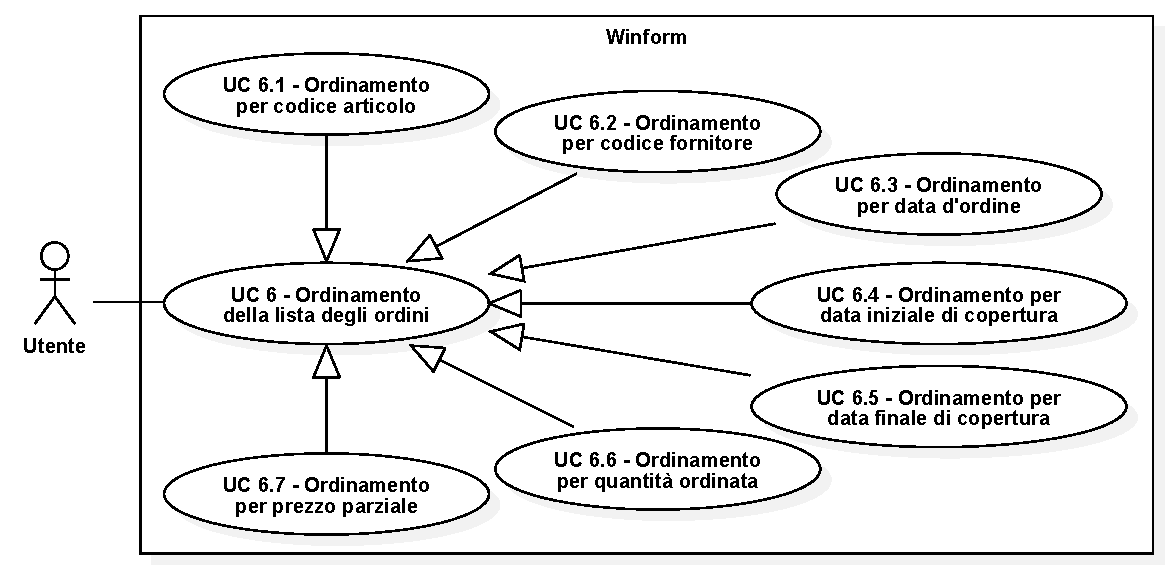
\includegraphics[width=0.95\columnwidth]{usecase/UC 6.pdf} 
    \caption{UC 6 - Ordinamento della lista degli ordini}
\end{figure}
\begin{itemize}

	\item \textbf{Attori primari: }
		\begin{itemize}
			\item Utente.
		\end{itemize}

	\item \textbf{Precondizione: }\\[0.3cm]
		L'utente visualizza correttamente la lista degli ordini.

	\item \textbf{Scenario principale: }
		\begin{enumerate}
			\item L'utente sceglie l'ordinamento da applicare alla lista.
		\end{enumerate}
		

	\item \textbf{Postcondizione: }\\[0.3cm]
		L'utente visualizza correttamente tutti gli elementi ordinati secondo la sua scelta.
    
    \item \textbf{Generalizzazioni: }
        \begin{itemize}
            \item Ordinamento per codice articolo (\hyperref[uc:ordinamento-codice-articolo]{UC 6.1});
            \item Ordinamento per codice fornitore (\hyperref[uc:ordinamento-codice-fornitore]{UC 6.2});
            \item Ordinamento per data d'ordine (\hyperref[uc:ordinamento-data-ordine]{UC 6.3});
            \item Ordinamento per data previsione inizio copertura (\hyperref[uc:ordinamento-data-iniziale-copertura]{UC 6.4});
            \item Ordinamento per data previsione fine copertura (\hyperref[uc:ordinamento-data-finale-copertura]{UC 6.5});
            \item Ordinamento per quantità ordinata (\hyperref[uc:ordinamento-quantita-ordinata]{UC 6.6});
            \item Ordinamento per prezzo parziale (\hyperref[uc:ordinamento-prezzo-parziale-ord]{UC 6.7}).
        \end{itemize}
\end{itemize}

\vspace{0.4cm}

\noindent \textbf{\large UC 6.1 - Ordinamento per codice articolo }
\label{uc:ordinamento-codice-articolo}
\begin{itemize}

	\item \textbf{Attori primari: }
		\begin{itemize}
			\item Utente.
		\end{itemize}

	\item \textbf{Precondizione: }\\[0.3cm]
		L'utente visualizza correttamente la lista degli ordini.
\item \textbf{Scenario principale: }
		\begin{enumerate}
			\item L'utente ordina la lista per codice articolo.
		\end{enumerate}
		

	\item \textbf{Postcondizione: }\\[0.3cm]
		L'utente visualizza correttamente tutti gli elementi ordinati rispetto al codice articolo.

\end{itemize}

\vspace{0.4cm}

\noindent \textbf{\large UC 6.2 - Ordinamento per codice fornitore }
\label{uc:ordinamento-codice-fornitore}
\begin{itemize}

	\item \textbf{Attori primari: }
		\begin{itemize}
			\item Utente.
		\end{itemize}

	\item \textbf{Precondizione: }\\[0.3cm]
		L'utente visualizza correttamente la lista degli ordini.

	\item \textbf{Scenario principale: }
		\begin{enumerate}
			\item L'utente ordina la lista per codice fornitore.
		\end{enumerate}
		

	\item \textbf{Postcondizione: }\\[0.3cm]
		L'utente visualizza correttamente tutti gli elementi ordinati rispetto al codice fornitore.

\end{itemize}

\vspace{0.4cm}

\noindent \textbf{\large UC 6.3 - Ordinamento per data d'ordine }
\label{uc:ordinamento-data-ordine}
\begin{itemize}

	\item \textbf{Attori primari: }
		\begin{itemize}
			\item Utente.
		\end{itemize}

	\item \textbf{Precondizione: }\\[0.3cm]
		L'utente visualizza correttamente la lista degli ordini.

	\item \textbf{Scenario principale: }
		\begin{enumerate}
			\item L'utente ordina la lista per data d'ordine.
		\end{enumerate}
		

	\item \textbf{Postcondizione: }\\[0.3cm]
		L'utente visualizza correttamente tutti gli elementi ordinati rispetto alla data d'ordine.

\end{itemize}

\vspace{0.4cm}

\noindent \textbf{\large UC 6.4 - Ordinamento per data iniziale di copertura }
\label{uc:ordinamento-data-iniziale-copertura}
\begin{itemize}

	\item \textbf{Attori primari: }
		\begin{itemize}
			\item Utente.
		\end{itemize}

	\item \textbf{Precondizione: }\\[0.3cm]
		L'utente visualizza correttamente la lista degli ordini.

	\item \textbf{Scenario principale: }
		\begin{enumerate}
			\item L'utente filtra uno o più ordini per data iniziale di copertura.
		\end{enumerate}
		

	\item \textbf{Postcondizione: }\\[0.3cm]
		L'utente visualizza correttamente tutti gli elementi ordinati rispetto alla data iniziale di copertura.

\end{itemize}

\vspace{0.4cm}

\noindent \textbf{\large UC 6.5 - Ordinamento per data finale di copertura}
\label{uc:ordinamento-data-finale-copertura}
\begin{itemize}

	\item \textbf{Attori primari: }
		\begin{itemize}
			\item Utente.
		\end{itemize}

	\item \textbf{Precondizione: }\\[0.3cm]
		L'utente visualizza correttamente la lista degli ordini.

	\item \textbf{Scenario principale: }
		\begin{enumerate}
			\item L'utente filtra uno o più ordini per data finale di copertura.
		\end{enumerate}
		

	\item \textbf{Postcondizione: }\\[0.3cm]
		L'utente visualizza correttamente tutti gli elementi ordinati rispetto alla data finale di copertura.

\end{itemize}

\vspace{0.4cm}

\noindent \textbf{\large UC 6.6 - Ordinamento per quantità ordinata}
\label{uc:ordinamento-quantita-ordinata}
\begin{itemize}

	\item \textbf{Attori primari: }
		\begin{itemize}
			\item Utente.
		\end{itemize}

	\item \textbf{Precondizione: }\\[0.3cm]
		L'utente visualizza correttamente la lista degli ordini.

	\item \textbf{Scenario principale: }
		\begin{enumerate}
			\item L'utente filtra uno o più ordini per quantità ordinata.
		\end{enumerate}
		

	\item \textbf{Postcondizione: }\\[0.3cm]
		L'utente visualizza correttamente tutti gli elementi ordinati rispetto alla quantità ordinata.

\end{itemize}

\vspace{0.4cm}

\noindent \textbf{\large UC 6.7 - Ordinamento per prezzo parziale}
\label{uc:ordinamento-prezzo-parziale-ord}
\begin{itemize}

	\item \textbf{Attori primari: }
		\begin{itemize}
			\item Utente.
		\end{itemize}

	\item \textbf{Precondizione: }\\[0.3cm]
		L'utente visualizza correttamente la lista degli ordini.

	\item \textbf{Scenario principale: }
		\begin{enumerate}
			\item L'utente ordina gli elementi rispetto al prezzo parziale.
		\end{enumerate}
		

	\item \textbf{Postcondizione: }\\[0.3cm]
		L'utente visualizza correttamente tutti gli elementi ordinati rispetto al prezzo parziale.

\end{itemize}

\vspace{0.4cm}

\section{Tracciamento dei requisiti}

\noindent Da un'attenta analisi dei requisiti e degli \textit{use case} effettuata sul progetto è stata stilata la tabella che traccia i requisiti in rapporto agli \textit{use case}.\\
Sono stati individuati diversi tipi di requisiti e si è dunque utilizzato un codice identificativo univoco per distinguerli.\\
Il codice dei requisiti è così strutturato:
\begin{center}
    \textbf{R<NumeroRequisito>-<Tipo>-<Classificazione>}
\end{center}
In particolare il tipo può assumere 4 valori, quali:
\begin{itemize}
    \item \textbf{F} $=$ funzionale;
    \item \textbf{Q} $=$ qualitativo;
    \item \textbf{P} $=$ performance;
    \item \textbf{V} $=$ vincolo.
\end{itemize}
Per quanto riguarda la classificazione, invece, si hanno 3 valori possibili:
\begin{itemize}
    \item \textbf{O} $=$ obbligatorio;
    \item \textbf{D} $=$ desiderabile;
    \item \textbf{F} $=$ facoltativo.
\end{itemize}
Nelle tabelle \ref{tab:requisiti-funzionali}, \ref{tab:requisiti-qualitativi}, \ref{tab:requisiti-di-performance} e \ref{tab:requisiti-di-vincolo} suddivise per tipo sono riassunti i requisiti e il loro tracciamento con gli \textit{use case} delineati in fase di analisi.

%comando arraystretch
\renewcommand{\arraystretch}{1.6}

% tab funzionali

\begin{center}
\rowcolors{2}{lightest-grayest}{white}
\begin{longtable}{|p{2cm}|p{7cm}|p{2cm}|}
\caption{Tabella del tracciamento dei requisiti funzionali}
\label{tab:requisiti-funzionali}
\\ \hline
\rowcolor{lighter-grayer}
\centering \textbf{Requisito} & \centering \textbf{Descrizione} & \centering \textbf{\textit{Use Case}} \arraybackslash \\
\hline 
\req{R1-F-O}{L'utente deve poter inserire i dati necessari per l'ottimizzazione}{\hyperref[uc:inserimento-dati]{UC1}}
\req{R2-F-O}{L'utente deve poter inserire la data di inizio previsione}{\hyperref[uc:inserimento-data-inizio-prev]{UC1.1}}
\req{R3-F-O}{L'utente deve poter inserire la data di fine previsione}{\hyperref[uc:inserimento-data-fine-prev]{UC1.2}}
\req{R4-F-O}{L'utente deve poter essere avvisato dell'errore di inserimento della data di inizio previsione}{\hyperref[uc:err-inserimento-data-inizio-prev]{UC1.3}}
\req{R5-F-O}{L'utente deve poter essere avvisato dell'errore di inserimento della data di fine previsione}{\hyperref[uc:err-inserimento-data-fine-prev]{UC1.4}}
\req{R6-F-O}{L'utente deve poter iniziare l'analisi di ottimizzazione}{\hyperref[uc:inizio-analisi-ottimizzazione]{UC2}}
\req{R7-F-O}{L'utente deve poter visualizzare i risultati}{\hyperref[uc:visualizzazione-risultati]{UC3}}
\req{R8-F-O}{L'utente deve poter visualizzare il totale non ottimizzato}{\hyperref[uc:visualizzazione-totale-non-ottimizzato]{UC3.1}}
\req{R9-F-O}{L'utente deve poter visualizzare il totale ottimizzato}{\hyperref[uc:visualizzazione-totale-ottimizzato]{UC3.2}}
\req{R10-F-O}{L'utente deve poter visualizzare lo scostamento tra i totali}{\hyperref[uc:visualizzazione-scostamento-percentuale-totali]{UC3.3}}
\req{R11-F-O}{L'utente deve poter visualizzare la lista degli ordini in maniera decrescente rispetto al codice articolo}{\hyperref[uc:visualizzazione-lista-ordini]{UC4}}
\req{R12-F-O}{L'utente deve poter visualizzare un singolo ordine della lista}{\hyperref[uc:visualizzazione-singolo-ordine]{UC4.1}}
\req{R13-F-O}{L'utente deve poter visualizzare il codice articolo di un ordine}{\hyperref[uc:visualizzazione-codice-articolo]{UC4.1.1}}
\req{R14-F-O}{L'utente deve poter visualizzare il codice fornitore di un ordine}{\hyperref[uc:visualizzazione-codice-fornitore]{UC4.1.2}}
\req{R15-F-O}{L'utente deve poter visualizzare la data d'ordine di un ordine}{\hyperref[uc:visualizzazione-data-ordine]{UC4.1.3}}
\req{R16-F-O}{L'utente deve poter visualizzare la data iniziale di copertura di un ordine}{\hyperref[uc:visualizzazione-data-iniziale-copertura]{UC4.1.4}}
\req{R17-F-O}{L'utente deve poter visualizzare la data finale di copertura di un ordine}{\hyperref[uc:visualizzazione-data-finale-copertura]{UC4.1.5}}
\req{R18-F-O}{L'utente deve poter visualizzare la quantità ordinata di un ordine}{\hyperref[uc:visualizzazione-quantita-ordinata]{UC4.1.6}}
\req{R19-F-O}{L'utente deve poter visualizzare il prezzo parziale di un ordine}{\hyperref[uc:visualizzazione-prezzo-parziale-ord]{UC4.1.7}}
\req{R20-F-O}{L'utente deve poter filtrare la lista}{\hyperref[uc:filtraggio-dati]{UC5}}
\req{R21-F-O}{L'utente deve poter filtrare la lista tramite una ricerca generica}{\hyperref[uc:filtraggio-ricerca-generica]{UC5.1}}
\req{R22-F-O}{L'utente deve poter filtrare la lista per codice articolo}{\hyperref[uc:filtraggio-codice-articolo]{UC5.2}}
\req{R23-F-O}{L'utente deve poter filtrare la lista per codice fornitore}{\hyperref[uc:filtraggio-codice-fornitore]{UC5.3}}
\req{R24-F-O}{L'utente deve poter filtrare la lista per data d'ordine}{\hyperref[uc:filtraggio-data-ordine]{UC5.4}}
\req{R25-F-O}{L'utente deve poter filtrare la lista per data iniziale di copertura}{\hyperref[uc:filtraggio-data-iniziale-copertura]{UC5.5}}
\req{R26-F-O}{L'utente deve poter filtrare la lista per data finale di copertura}{\hyperref[uc:filtraggio-data-finale-copertura]{UC5.6}}
\req{R27-F-O}{L'utente deve poter filtrare la lista per quantità ordinata}{\hyperref[uc:filtraggio-quantita-ordinata]{UC5.7}}
\req{R28-F-O}{L'utente deve poter filtrare la lista per prezzo parziale}{\hyperref[uc:filtraggio-prezzo-parziale-ord]{UC5.8}}
\req{R29-F-O}{L'utente deve poter ordinare la lista degli ordini}{\hyperref[uc:ordinamento-elementi-lista]{UC6}}
\req{R30-F-O}{L'utente deve poter ordinare la lista rispetto al codice articolo}{\hyperref[uc:ordinamento-codice-articolo]{UC6.1}}
\req{R31-F-O}{L'utente deve poter ordinare la lista rispetto al codice fornitore}{\hyperref[uc:ordinamento-codice-fornitore]{UC6.2}}
\req{R32-F-O}{L'utente deve poter ordinare la lista rispetto alla data d'ordine}{\hyperref[uc:ordinamento-data-ordine]{UC6.3}}
\req{R33-F-O}{L'utente deve poter ordinare la lista rispetto alla data iniziale di copertura}{\hyperref[uc:ordinamento-data-iniziale-copertura]{UC6.4}}
\req{R34-F-O}{L'utente deve poter ordinare la lista rispetto alla data finale di copertura}{\hyperref[uc:ordinamento-data-finale-copertura]{UC6.5}}
\req{R35-F-O}{L'utente deve poter ordinare la lista rispetto alla quantità ordinata}{\hyperref[uc:ordinamento-quantita-ordinata]{UC6.6}}
\req{R36-F-O}{L'utente deve poter ordinare la lista rispetto al prezzo parziale}{\hyperref[uc:ordinamento-prezzo-parziale-ord]{UC6.7}}
\end{longtable}
\end{center}%

\vspace*{\fill}

%tab qualità
\begin{center}
\rowcolors{2}{lightest-grayest}{white}
\begin{longtable}{|p{2cm}|p{7cm}|p{2cm}|}
\caption{Tabella del tracciamento dei requisiti qualitativi}
\label{tab:requisiti-qualitativi}
\\ \hline
\rowcolor{lighter-grayer}
\centering \textbf{Requisito} & \centering \textbf{Descrizione} & \centering \textbf{\textit{Use Case}} \arraybackslash \\
\hline 
\req{R37-Q-O}{Deve essere redatto un documento che descrive l'architettura del modulo}{-}
\req{R38-Q-O}{Deve essere redatto un documento che spieghi le scelte implementative effettuate}{-}
\req{R39-Q-O}{Il codice deve essere documentato tramite commenti}{-}
\req{R40-Q-D}{L'algoritmo finale scelto deve generare dei \textit{log} di chiamata per manutenzioni future}{-}
\req{R41-Q-D}{L'algoritmo di ottimizzazione deve essere estensibile}{-}
\req{R42-Q-D}{I \textit{test} devono coprire il 60\% del codice}{-}
\req{R43-Q-D}{L'algoritmo utilizza differenti tecniche di ottimizzazione}{-}
\req{R44-Q-F}{L'algoritmo utilizza il \textit{multithreading} per cercare più soluzioni ammissibili}{-}
\end{longtable}
\end{center}%

\vspace*{\fill}

\newpage

%tab performance
\begin{center}
\rowcolors{2}{lightest-grayest}{white}
\begin{longtable}{|p{2cm}|p{7cm}|p{2cm}|}
\caption{Tabella del tracciamento dei requisiti di performance}
\label{tab:requisiti-di-performance}
\\ \hline
\rowcolor{lighter-grayer}
\centering \textbf{Requisito} & \centering \textbf{Descrizione} & \centering \textbf{\textit{Use Case}} \arraybackslash \\
\hline 
\req{R45-P-O}{L'algoritmo di ottimizzazione deve restituire un risultato entro 10 minuti dal tempo di lancio dello stesso}{-}
\end{longtable}
\end{center}%

%tab vincolo
\begin{center}
\rowcolors{2}{lightest-grayest}{white}
\begin{longtable}{|p{2cm}|p{7cm}|p{2cm}|}
\caption{Tabella del tracciamento dei requisiti di vincolo}
\label{tab:requisiti-di-vincolo}
\\ \hline
\rowcolor{lighter-grayer}
\centering \textbf{Requisito} & \centering \textbf{Descrizione} & \centering \textbf{\textit{Use Case}} \arraybackslash \\
\hline  
\req{R46-V-O}{La \textit{form} deve essere eseguita sull'ambiente di esecuzione \textit{.NET Framework}}{-}
\req{R47-V-O}{La \textit{form} e l'algoritmo devono essere codificate in $C\#$}{-}
\req{R48-V-O}{La versione utilizzata di $C\#$ deve essere $7.3$}{-}
\req{R49-V-O}{La versione utilizzata di \textit{.NET Framework} deve essere $4.8$}{-}
\req{R50-V-O}{L'algoritmo finale deve fonire una soluzione \gls{ammissibileg}}{-}
\end{longtable}
\end{center}%

\begin{center}
	\rowcolors{2}{lightest-grayest}{white}
	\begin{longtable}{|p{2.5cm}|p{2.5cm}|p{2.5cm}|p{2.5cm}|}
	\caption{Riepilogo dei requisiti}
	\label{tab:requisiti-riepilogo}
	\\ \hline
	\rowcolor{lighter-grayer}
	\centering \textbf{Tipo} & \centering \textbf{Obbligatori} & \centering \textbf{Desiderabili} & \centering \textbf{Facoltativi}\arraybackslash \\
	\hline  
	\reqsum{Funzionali}{36}{0}{0}
	\reqsum{Qualitativi}{3}{4}{1}
	\reqsum{Prestazionali}{1}{0}{0}
	\reqsum{Vincolo}{5}{0}{0}
	\end{longtable}
\end{center}%